\documentclass[12pt,twoside]{article}
%%%%%%%%%%%%%%%%%%%%%%%%%%%%%%%%%%%%%%%%%%%%%%%%%%%%%%%%%%%%%
% Meta informations:
\newcommand{\trauthor}{Peter W\"uppen, Alvin Rindra Fazrie}
\newcommand{\trtype}{Seminar Paper Outline} %{Seminararbeit} %{Proseminararbeit}
\newcommand{\trcourse}{Bio-Inspired Artificial Intelligence}
\newcommand{\trtitle}{Interactive Reinforcement Learning: Learning with Advice}
\newcommand{\trmatrikelnummer}{605308, 6641834}
\newcommand{\tremail}{5wueppen@informatik.uni-hamburg.de \\ 4fazrie@informatik.uni-hamburg.de}
\newcommand{\trarbeitsbereich}{Knowledge Technology, WTM}
\newcommand{\trdate}{11.11.2015}

%%%%%%%%%%%%%%%%%%%%%%%%%%%%%%%%%%%%%%%%%%%%%%%%%%%%%%%%%%%%%
% Languages:

% Falls die Ausarbeitung in Deutsch erfolgt:
% \usepackage[german]{babel}
% \usepackage[T1]{fontenc}
% \usepackage[latin1]{inputenc}
% \usepackage[latin9]{inputenc}	 				
% \selectlanguage{german}

% If the thesis is written in English:
\usepackage[english]{babel} 						
\selectlanguage{english}

%%%%%%%%%%%%%%%%%%%%%%%%%%%%%%%%%%%%%%%%%%%%%%%%%%%%%%%%%%%%%
% Bind packages:
\usepackage{acronym}                    % Acronyms
\usepackage{algorithmic}				    % Algorithms and Pseudocode
\usepackage{algorithm}									% Algorithms and Pseudocode
\algsetup{linenosize=\tiny}
\usepackage{regexpatch}

\usepackage{etoolbox}
\AtBeginEnvironment{algorithm}{\setstretch{0.5}}

\makeatletter
\xpatchcmd{\algorithmic}{\labelsep 0.5em}{\labelsep 1.5em}{\typeout{Success!}}{\typeout{Oh dear!}}
\makeatother

\usepackage{enumitem}
\setlist{nosep}

\usepackage{setspace}
\usepackage{amsfonts}                   % AMS Math Packet (Fonts)
\usepackage{amsmath}                    % AMS Math Packet
\usepackage{amssymb}                    % Additional mathematical symbols
\usepackage{amsthm}
\usepackage{booktabs}                   % Nicer tables
%\usepackage[font=small,labelfont=bf]{caption} % Numbered captions for figures
\usepackage{color}                      % Enables defining of colors via \definecolor
\definecolor{uhhRed}{RGB}{254,0,0}		  % Official Uni Hamburg Red
\definecolor{uhhGrey}{RGB}{122,122,120} % Official Uni Hamburg Grey
\usepackage{fancybox}                   % Gleichungen einrahmen
\usepackage{fancyhdr}		
\usepackage{wrapfig}								% Packet for nicer headers
%\usepackage{fancyheadings}             % Nicer numbering of headlines

%\usepackage[outer=3.35cm]{geometry} 	  % Type area (size, margins...) !!!Release version
%\usepackage[outer=2.5cm]{geometry} 		% Type area (size, margins...) !!!Print version
%\usepackage{geometry} 									% Type area (size, margins...) !!!Proofread version
\usepackage[outer=3.15cm]{geometry} 	  % Type area (size, margins...) !!!Draft version
\geometry{a4paper,body={5.8in,9in}}

\usepackage{graphicx}                   % Inclusion of graphics
%\usepackage{latexsym}                  % Special symbols
\usepackage{longtable}									% Allow tables over several parges
\usepackage{listings}                   % Nicer source code listings
\usepackage{multicol}										% Content of a table over several columns
\usepackage{multirow}										% Content of a table over several rows
\usepackage{rotating}										% Alows to rotate text and objects
\usepackage[hang]{subfigure}            % Allows to use multiple (partial) figures in a fig
%\usepackage[font=footnotesize,labelfont=rm]{subfig}	% Pictures in a floating environment
\usepackage{tabularx}										% Tables with fixed width but variable rows
\usepackage{url,xspace,boxedminipage}   % Accurate display of URLs

%%%%%%%%%%%%%%%%%%%%%%%%%%%%%%%%%%%%%%%%%%%%%%%%%%%%%%%%%%%%%
% Configurationen:

\hyphenation{whe-ther} 									% Manually use: "\-" in a word: Staats\-ver\-trag

%\lstloadlanguages{C}                   % Set the default language for listings
\DeclareGraphicsExtensions{.pdf,.svg,.jpg,.png,.eps} % first try pdf, then eps, png and jpg
\graphicspath{{./src/}} 								% Path to a folder where all pictures are located
\pagestyle{fancy} 											% Use nicer header and footer

% Redefine the environments for floating objects:
\setcounter{topnumber}{3}
\setcounter{bottomnumber}{2}
\setcounter{totalnumber}{4}
\renewcommand{\topfraction}{0.9} 			  %Standard: 0.7
\renewcommand{\bottomfraction}{0.5}		  %Standard: 0.3
\renewcommand{\textfraction}{0.1}		  	%Standard: 0.2
\renewcommand{\floatpagefraction}{0.8} 	%Standard: 0.5

% Tables with a nicer padding:
\renewcommand{\arraystretch}{1.2}

%%%%%%%%%%%%%%%%%%%%%%%%%%%%
% Additional 'theorem' and 'definition' blocks:
\theoremstyle{plain}
\newtheorem{theorem}{Theorem}[section]
%\newtheorem{theorem}{Satz}[section]		% Wenn in Deutsch geschrieben wird.
\newtheorem{axiom}{Axiom}[section] 	
%\newtheorem{axiom}{Fakt}[chapter]			% Wenn in Deutsch geschrieben wird.
%Usage:%\begin{axiom}[optional description]%Main part%\end{fakt}

\theoremstyle{definition}
\newtheorem{definition}{Definition}[section]

%Additional types of axioms:
\newtheorem{lemma}[axiom]{Lemma}
\newtheorem{observation}[axiom]{Observation}

%Additional types of definitions:
\theoremstyle{remark}
%\newtheorem{remark}[definition]{Bemerkung} % Wenn in Deutsch geschrieben wird.
\newtheorem{remark}[definition]{Remark} 

%%%%%%%%%%%%%%%%%%%%%%%%%%%%
% Provides TODOs within the margin:
\newcommand{\TODO}[1]{\marginpar{\emph{\small{{\bf TODO: } #1}}}}

%%%%%%%%%%%%%%%%%%%%%%%%%%%%
% Abbreviations and mathematical symbols
\newcommand{\modd}{\text{ mod }}
\newcommand{\RS}{\mathbb{R}}
\newcommand{\NS}{\mathbb{N}}
\newcommand{\ZS}{\mathbb{Z}}
\newcommand{\dnormal}{\mathit{N}}
\newcommand{\duniform}{\mathit{U}}

\newcommand{\erdos}{Erd\H{o}s}
\newcommand{\renyi}{-R\'{e}nyi}
%%%%%%%%%%%%%%%%%%%%%%%%%%%%%%%%%%%%%%%%%%%%%%%%%%%%%%%%%%%%%
% Document:
\begin{document}
\renewcommand{\headheight}{14.5pt}

\fancyhead{}
\fancyhead[LE]{ \slshape \trauthor}
\fancyhead[LO]{}
\fancyhead[RE]{}
\fancyhead[RO]{ \slshape \trtitle}

%%%%%%%%%%%%%%%%%%%%%%%%%%%%
% Cover Header:
\begin{titlepage}
	\begin{flushleft}
		Universit\"at Hamburg\\
		Department Informatik\\
		\trarbeitsbereich\\
	\end{flushleft}
	\vspace{3.5cm}
	\begin{center}
		\huge \trtitle\\
	\end{center}
	\vspace{3.5cm}
	\begin{center}
		\normalsize\trtype\\
		[0.2cm]
		\Large\trcourse\\
		[1.5cm]
		\Large \trauthor\\
		[0.2cm]
		\normalsize Matr.Nr. \trmatrikelnummer\\
		[0.2cm]
		\normalsize\tremail\\
		[1.5cm]
		\Large \trdate
	\end{center}
	\vfill
\end{titlepage}

	%backsite of cover sheet is empty!
\thispagestyle{empty}
\hspace{1cm}
\newpage

%%%%%%%%%%%%%%%%%%%%%%%%%%%%
% Abstract:

% Abstract gives a brief summary of the main points of a paper:
\section*{Abstract}


Interaction between Artificial Intelligence and humans has been growing to be a vital part in daily life in the past decade. Reinforcement Learning has become one of the fundamental topics for scientists in the field of robotic and machine learning. In this paper, we introduce the basic concepts of reinforcement learning and expand on the idea of external interaction to support the learning process. To this end, we introduce a number of proposed approaches to interactive RL and discuss their implications. Finally, we attempt to implement  an effective advice strategy for interactive RL based on an existing simulated scenario of a domestic cleaning task presented in \cite{cruz2014improving}.

% Lists:
\setcounter{tocdepth}{2} 					% depth of the table of contents (for Seminars 2 is recommented)
\tableofcontents
\pagenumbering{arabic}
\clearpage



%%%%%%%%%%%%%%%%%%%%%%%%%%%%
% Content:

% the actual content, usually separated over a number of sections
% each section is assigned a label, in order to be able to put a
% crossreference to it

\section{Introduction}
\label{sec:introduction}
  
Current technology recently has been built with Artificial Intelligence that humans could interact with. Interaction between humans and AI is getting popular in part of daily life e.g., drone, autonomous car, and even video games since AI player could make the games becoming more impressive and challenging. In this regards, AI player should implement a learning approach which could make them learn acting unpredicted scenarios through another AI and humans.

Interactive Reinforcement learning has proven to be great potential in adapting and learning multiple tasks especially. The idea behind RL is to respond according to a set of desired actions and to continuously observe the current and potential environment. With a reinforcement learning approach, the agent explores the environment
around it with an aim to maximize the rewards that it could gain by interacting
with the environment. The core of the reinforcement learning concept is based on Markov decision process(MDP). 



\section{Reinforcement Learning Basics}

In these decades, several fields have already implemented Reinforcement learning method and it is proven to show great performance in machine learning paradigms. In this section we will provide a brief understanding of reinforcement learning, the basic setup, value function and how to find the optimal policies.

Reinforcement learning is a learning mechanism where an agent learns to observe the environment continuously and respond with a set of allowed actions within the environment. The agent once performs the desired action will receive a feedback from the environment. Each of the actions performed by the agent is selected based on the decision according to an internal decision-making policy where the policy is simply a probability of an action $a$ being taken for a given $s$. 

The feedback given to the agent will be in the form of a scalar reward from the RL framework, which will be decided by a reward function. The reward could diverse based on what kind of agent behavior is expected and it will be utilized as a factor to update the action selection policy to gain an optimal policy. In other terms the agent’s ultimate goal is to achieve an optimal behavior by learning the optimal action for each state.

\subsection{Basic Setup}


Reinforcement Learning is arranged in certain steps continuously, the basic step reinforcement learning model can be seen as listed below:


\begin{wrapfigure}{r}{0.6\textwidth}
  \begin{center}
    \includegraphics[width=0.6\textwidth]{rl.png}
  \end{center}
  \caption{Reinforcement learning diagram showing an agent's interaction with its environment \cite{Sutton1998introduction}.}
  \label{rl}
\end{wrapfigure}

\begin{enumerate}
	\item Observe state, $s_t$
	\item Decide on an action, $a_t$
	\item Perform action
	\item Get the reward	
	\item Observe new state, $s_{t+1}$
	\item Update policy based on the given reward
	\item Repeat
\end{enumerate}
The model has an aim to find a control policy which will maximize the observed rewards for the agent.

In RL an agent will face a certain state each time $(s_t \in S)$ and in the current state the agent needs to select a possible action and then perform it $(a_t \in A(s_t))$. Once the action has been done by the agent, a positive or a negative value as a reward will be provided by the environment $(r_t)$ and the following state $(s_{t+1})$ to the agent in the next step \cite{Sutton1998introduction}.

Policy maps a state to an action through the process. $(\pi_t(s_t, a_t))$; moreover, learning process is changing the policy in order to gain experience from the environment and the main goal of agent is maximizing the accumulated reward.\cite{Sutton1998introduction}.
The basic model of standard reinforcement learning is depicted in figure 1.


Markov Decision Process is the basis of core components for Reinforcement Learning, and several core components which define the Reinforcement Learning could be formalized as follows \cite{baier2007learning}:
\begin{itemize}
\item State space, denoted by $s \in S$, is a discrete set of environment states.

\item Action space, denoted by $a \in A$, is a discrete set of actions from the environment's agent.

\item Reward function, denoted by $r : S \times A \rightarrow \mathbb{R}$, is a function which turns each transition for a given state into a scalar value.

\item State Transition function, denoted by $\delta : S \times A \rightarrow S$, is a  function which gives the potential state $s'$ when the action $a$ is conducted.

\item Policy, denoted by $\pi$, is a function which specifies the agents behavior. It maps the action to be taken for each given state. i.e., $\pi_t : S \rightarrow A$, where S is the environment state set and A is the agent action.

\item State value function, denoted by $V^\pi : S \rightarrow \mathbb{R}$, is a function that will be used to obtain the highest reward as the agent will always try to learn. It specifies the value for each state and maps the state to the reward an agent can expect to accumulate. 
\end{itemize}

\subsection{Q-Value functions}

In Reinforcement Learning, the agent needs to achieve its main goal which is to take an action in each step that could maximize the total reward. The total reward estimation which an agent could obtain by performing an action in the current state (action-value pairs) could be calculated with the equation below \cite{Sutton1998introduction}.


\begin{equation} \label{eq2}
Q^\pi(s,a) = E_\pi \{ \sum_{k=0}^{\infty} \gamma^k r_t + k +1 | s_t = s, a_t = a \}
\end{equation}


From the equation, it can be seen that $Q(s, a)$ is the state-action pairs value and $r_t$ is the action reward $a = a_t$ under the policy $\pi$ in the state $s = s_t$ . Moreover, $\gamma$ is discount rate of future actions influence $(0 \leq \gamma < 1)$. 

From that equation, the optimized estimation of state-action pairs
value can be formularized in equation below which is called Bellman Equation \cite{Sutton1998introduction}:

\begin{equation} \label{eq3}
Q^*(s,a) = \sum_{s'} P(s'|s,a) [r(s,a,s') + \gamma \max_{a'} Q(s',a')]
\end{equation}

In this equation, $Q ∗ (s, a)$ is the optimal function to do state-action pairs value estimation where $p$ is the probability to achieve the subsequent state $s' = s_t+1$ which is performed bey $a$ as an action in the current state $s$ and $a'$ representing the possible actions set in the future state $s'$ \cite{Sutton1998introduction}.
state action pair value.

\section{RL with Interactive Feedback}

The basic strategy of reinforcement learning is very closely related to how humans and animals initially learn to fulfill tasks and interact with their environment. However, human learning mechanisms have a clear advantage in the direct comparison: They do not exclusively work tediously by trial and error, but have helpful outside influences to guide learning. For example, imitation plays a big role as a direct transfer of behavior knowledge. Another important aspect is guidance during autonomous learning by having a knowledgeable other person give input on the learner's decisions, essentially teaching them crucial strategies to solve the task at hand. In this section, we will give a summary of some approaches that have been proposed to incorporate a teaching mechanism into reinforcement learning algorithms. We separate between agent advising, where an agent already trained for a certain task is used to speed up the learning process of a second one, and human advising which aims at using human rewards to achieve the same.

\subsection{Approaches for Agent Advising}

In \cite{Taylor2014reinforcement}, Taylor et al. discuss the viability of different strategies for having an agent teach another one about a certain task. Their chosen problem domain is the one of video games: By finding good teaching strategies between agents, they hope to transfer this knowledge into the construction of agents that can also teach humans effectively about games after autonomously learning about them themselves. According to the authors, this could reduce the amount of effort game developers have to put into creating specific training scenarios to teach new players about the game initially. \\
Taylor et al. propose two critical limitations to teaching algorithms in order to be able to transfer them towards human teaching later: The teaching and the learning agent must not be required to have the same state representation, and the teacher cannot give unlimited amount of advice. The first limitation seems obvious: A human player would obviously have a vastly different representation of the state of a game than an agent would despite having the same set of actions available to him. Their second limitation comes from the idea that humans have "limited patience and attention" (\cite{Taylor2014reinforcement}) for incoming advice. While this is certainly true, the bigger reason for not having unlimited advice in games is that many players play games partly because they want to figure them out themselves instead of just being guided through the process with no perceived decision making on their part. A game that took away this sense of self-accomplishment would probably be even less successful than one that let players figure out everything on their own.
To model this kind of limited advice, Taylor et al. introduce the notion of a "budget" $n$ available to the teacher. It is a fixed number and denotes how often the teacher is allowed to intervene during a learning episode of the student and suggest a certain action to them. This naturally lends itself to the question of how this budget is spent best and what criteria the teacher should look at to determine whether to help the student with a particular choice or not. \\
Taylor et al. propose and compare five different strategies for spending the teaching budget which will be briefly summarized here.

\subsubsection{Early advising}

Early advising simply lets the teaching agent spend its budget as soon as possible, so in the first $n$ states the student encounters. The intuition behind this approach is that it might be best to help the student most in the beginning, when they still know very little about the task \cite{Taylor2014reinforcement}.


\begin{algorithm}[H]
  \algsetup{linenosize=\tiny}
  \scriptsize
  \begin{enumerate}
	\linespread{1.0}
	\item \textbf{procedure} EarlyAdvising ($\pi, n$). 
	\item \qquad \textbf{for} each student state $s$ \textbf do
	\item \qquad \qquad \textbf{if} $n > 0$ \textbf{then}
	\item \qquad \qquad \qquad $n \leftarrow n - 1$
	\item \qquad \qquad \qquad Advice $\pi(s)$
	\item \qquad \qquad \textbf{end if}
	\item \qquad \textbf{end for}
	\item \textbf{end procedure}
	\end{enumerate}
  	\caption{Early Advising}
\end{algorithm}


\subsubsection{Alternate advising}

Alternate advising follows the same logic as early advising, but attempts to space out the advice more evenly to be able to help for a longer period of the episode. Instead of giving advice in every step, alternate advising as proposed by Taylor et al. gives advice every $m$th step, so that the advice budget is finally exhausted after $nm$ steps.


\subsubsection{Importance advising}

Importance advising takes into the account the fact that giving advice may be more crucial in some situations than in others. To that end, Taylor et al. propose an importance function $I(s)$ that maps states to real values and indicates how important it is to get the decision about the action right in this particular state. Multiple implementations of this importance function are suggested, including measuring the maximal difference between Q-values for the state as well as their variance and absolute deviation (\cite{Taylor2014reinforcement}). The latter two probably produce more consistent results, as they take into more Q-values than the two most extreme ones.
The teacher then evaluates this function in every state and depending on if it exceeds a certain threshold or not, decides whether or not to give advice to the student in this step.


\begin{algorithm}[H]
  \algsetup{linenosize=\tiny}
  \scriptsize
  \begin{enumerate}
\setstretch{1.0}
	\item \textbf{procedure} ImportanceAdvising ($\pi, n, t$). 
	\item \qquad \textbf{for} each student state $s$ \textbf do
	\item \qquad \qquad \textbf{if} $n > 0$ and $I(s) \geq t $ \textbf{then}
	\item \qquad \qquad \qquad $n \leftarrow n - 1$
	\item \qquad \qquad \qquad Advice $\pi(s)$
	\item \qquad \qquad \textbf{end if}
	\item \qquad \textbf{end for}
	\item \textbf{end procedure}
\end{enumerate}
  	\caption{Importance Advising}
\end{algorithm}



\subsubsection{Mistake correcting}

Mistake correcting differs substantially from the other strategies as it takes into the account the decision the student makes autonomously before deciding whether to give advice or not. The idea behind this is that a sparse advice budget should not be spent when the student is already making the right decision. The downside of this is another layer of communication, as students would need to inform the teacher about their decision first and wait for potential advice before carrying out any actions (\cite{Taylor2014reinforcement}). Advice is thus dependent both on the action taken by the student as well the importance metric (both preconditions need to be fulfilled).
This restriction seems to be largely impracticable especially in the suggested problem domain, as players cannot be expected to announce their following actions and wait for feedback on every step of the way without completely eliminating their sense of flow.



\begin{algorithm}[H]
  \algsetup{linenosize=\tiny}
  \scriptsize
 \begin{enumerate}
	\item \textbf{procedure} MistakeCorrecting ($\pi, n, t$). 
	\item \qquad \textbf{for} each student state $s$ \textbf do
	\item \qquad \qquad Observe students announced action $a$
	\item \qquad \qquad \textbf{if} $n > 0$ and $I(s) \geq t $  and $a \neq \pi(s)$ \textbf{then}
	\item \qquad \qquad \qquad $n \leftarrow n - 1$
	\item \qquad \qquad \qquad Advice $\pi(s)$
	\item \qquad \qquad \textbf{end if}
	\item \qquad \textbf{end for}
	\item \textbf{end procedure}
\end{enumerate}
  	\caption{Mistake Correcting}
\end{algorithm}




\subsubsection{Predictive advising}

Predictive advising also aims at saving advice in cases where students are making the correct decisions by themselves, but instead of having them announce their actions prior to carrying them out, the teacher itself actually tries to learn about their behaviour and predict whether or not they would go wrong in certain states or not. To this end, the teacher uses the actions the student takes as training examples for a classifier that predicts future actions\cite{Taylor2014reinforcement}.
Obviously, this strategy can fail rather easily especially during the early stages of learning which might cause the teacher to give advice where none is needed, or even more crucial, miss good opportunities to speed up the learning process. Also, the reduced communication overhead is replaced by additional computation needed to constantly update the classifier. And finally, the training data for the classifier will always contain a good amount of noise since students will often go for unpredictable random exploration steps.

\begin{algorithm}[H]
  \algsetup{linenosize=\tiny}
  \scriptsize
 \begin{enumerate}
	\item \textbf{procedure} PredictiveAdvising ($\pi, n, t$). 
	\item \qquad \textbf{for} each student state $s$ \textbf do
	\item \qquad \qquad Predict students intended action $a$
	\item \qquad \qquad \textbf{if} $n > 0$ and $I(s) \geq t $  and $a \neq \pi(s)$ \textbf{then}
	\item \qquad \qquad \qquad $n \leftarrow n - 1$
	\item \qquad \qquad \qquad Advice $\pi(s)$
	\item \qquad \qquad \textbf{end if}
	\item \qquad \textbf{end for}
	\item \textbf{end procedure}
\end{enumerate}
  	\caption{Predictive Advising}
\end{algorithm}

\subsubsection{Experimental results}

Taylor et al. present experimental results for two independent examples for their approaches of interactive reinforcement learning. These are the arcade game Pac-Man as a whole as well as a specific sub-scenario from the real-time strategy game StarCraft (\cite{Taylor2014reinforcement}). They use different combinations of state representations between teachers and students as well as most of the different budgeting strategies for every combination to determine which seems to work best on the chosen examples. In particular, they examine the effects of having "smarter" agents with more refined state feature sets teach simpler ones as well as the other way around. \\
Their results show that in all cases and combinations, giving advice has significant statistical influence on performance metrics of the students like their average episode reward, in comparison to learning the task completely autonomously \cite{Taylor2014reinforcement}. The strategy of mistake correcting seems to be the most effective overall, as none of the different configurations let any other budgeting strategy outperform it in a statistically significant way. This comes as no surprise: Having knowledge about the students actions ahead of time obviously allows for powerful teaching strategies when on a strict budget. For the StarCraft example, Taylor et al. also tried a predictive approach which came very close in performance to the mistake correcting one \cite{Taylor2014reinforcement}, showcasing that the restrictive precondition of having the student communicate its choices prior to executing them can at least be partially circumvented. Importance advising showed a slight but mostly statistically significant deficit in performance in comparison to the previously mentioned strategies \cite{Taylor2014reinforcement}. Nevertheless, one has to consider that its runtime overhead is also much lower, since it only requires one evaluation of the importance function per time step. Lastly, both early and alternate advising on average performed significantly worse than the other strategies, but still represented a huge improvement over learning without any advice at all \cite{Taylor2014reinforcement}. Overall, this indicates a clear tradeoff between effectiveness and computational overhead of the teaching method. For the domain of video games, importance advising or predictive advising seem like the best options: Players won't mind much if they occasionally get advice that they didn't really need as long as it is helpful to them on average, while having to wait for feedback before being "allowed" to perform actions like with mistake correcting seems obstructive to the flow of the game and could give the player the feeling of not even making any relevant choices himself.

\subsection{Approaches for Human Advising}
Just like IRL can be applied to have autonomous agents teach humans about certain tasks, the opposite scenario is possible: Using human input to support an autonomous agent in learning a certain task. In \cite{thomaz2005real} and \cite{Thomaz2006reinforcement}, Thomaz et al. explore fundamental properties of such an interactive reinforcement learning task. Their goal is to find out in what ways humans want to teach an agent and thus how the agent should be set up to interpret the advice it gets in the most optimal way, so that eventually an ordinary person with no expert knowledge on the inner workings or learning procedures of an agent or robot could support it in learning a previously unknown task in a reasonable amount of time. To that end, they set up a simulated environment which they label "Sophie's Kitchen". It consists of a set of locations ($shelf$, $table$, $oven$, $agent$) and objects ($flour$, $eggs$, $spoon$, $bowl$, $tray$). Each Object is always in one of a set of object-specific states and belongs to exactly one location in the environment. Being in the $agent$ location symbolizes that an object is currently being carried by the agent. The agent's objective now is to interact with the objects in such a way that a certain goal state is reached, in this case it is supposed to bake a cake using the available ingredients and tools. To that end, it can move from location to location, pick up an object from its current location and drop down one currently in its possession, or use a carried object on one that is in the current location, possibly altering its object state. 
\\
In this environment, Thomaz et al. then use a Q-Learning agent to learn this task. Each step of the agent gives a slight negative reward to encourage finishing quickly, with the exception of the goal state with a high positive reward and the so-called catastrophic states in which the episode instantly terminates with a high negative one. The catastrophic states are ones from which the goal state cannot possibly be reached anymore. During its learning process, the agent and its actions are being visualized and a human trainer can influence the learning process at any point by giving manual reward to the agent on a scale from $-1$ to $1$. The trainer can choose to relate this reward to the state as a whole or to a certain object they want to select. The agent however always interprets the given reward as pertaining to the whole state they are currently in. Thomaz et al. then had 18 participants with no prior knowledge on the system or the underlying learning process try to teach the agent about the task (they were informed what actions needed to be taken to succeed). Specifically, they were instructed to use the reward signal exclusively as feedback for what the agent just did. One of the results of this experiment was the realization that the participants often tried to guide the agent towards future actions using the object-specific reward signal as opposed to just providing feedback with it. Based on this first observation, Thomaz et al. then implemented a second mechanism to support this behaviour by allowing the trainer to mark certain objects, supposedly to guide the agent's attention towards them. Internally, these messages were used to restrict the possible action space for the agent in the next step by only allowing to choose actions that were related to the currently marked object. In comparison to the previous setup of only having feedback available, the addition of the guidance option showed significantly improved results of the learning process both for expert users following a best-case protocol as well as for non-expert users. The authors conclude that interactive reinforcement learning approaches with human teachers should involve both feedback as well as guidance channels to improve the learning process as much as possible and to offer intuitive ways for humans to teach agents.
\\
While the logic of this approach is mostly sound, there are some logical pitfalls to consider, especially with the chosen environment for the conducted tests. The general purpose of reinforcement learning should be that an agent finds ways to accomplish a task even in cases where the solution is not obvious. If a teacher already has perfect knowledge of the task and the optimal sequence of actions to be taken, then letting an agent try to learn on its own instead of simply giving it an action protocol makes little sense. This can also be seen as part of the reason why the guidance-factor made such a big difference in this example: participants wanted to mostly guide the agents because they knew exactly what actions to perform in what order. The real application area of this approach however should be tasks where a teacher only knows about the task itself, but not in detail about what the agent specifically needs to do in order to fulfill it. This is a delicate balance: If there is too much prior knowledge, then reinforcement learning in general is not the most useful approach, if there is too little or no knowledge, then adding an interactive component will not make much of a difference. For their sample experiment, Thomaz et al. heavily leaned towards the former. Maybe if the task was set up in a way where it was not completely obvious for the participants to judge what to do next, their preferred style of teaching would actually have been to give feedback on the agents current state rather than to try and guide it towards future actions.

\section{Implementation}
In \cite{cruz2014improving}, Cruz et al. aim to find ways to improve the convergence speed of reinforcement learning algorithms by using two approaches: A concept of "affordances" which they introduce to restrict an agent's action space and a form of interactive RL where a previously trained agent is used to support the learning process of another one. In this paper, we will focus on discussing and improving the interactive elements of their approach. To this end, we introduce the algorithm and training scenario used in \cite{cruz2014improving} and propose possible changes to improve its interactive component.
\subsection{Description of the scenario and algorithm}
The scenario suggested in \cite{cruz2014improving} features a humanoid robot facing the task of cleaning a table in front of it. The table is separated into the two sides $left$ and $right$, both of which are initially dirty. There is a third location $home$ and two objects: a $cup$, initially located at $left$, and a sponge, initially located at $home$. The robot's arm with which the cleaning task is to be carried out also starts at the location $home$ and can perform the following actions: $get$ to pick up an object at its current location, $drop$ to drop the currently carried object, $go$ to move to any of the locations and $clean$ to attempt to clean the current location, using the object being carried. Many of the actions can lead to failure, like trying to $clean$ something with the $cup$ in hand or trying to clean a location that the cup is currently at. After cleaning, the robot is supposed to return the sponge to the $home$ position, which is the final goal state of the system. The reward for every state encountered is $-0.01$ to discourage redundant behaviour, with the exception of the goal state and the failure states, which reward $1$ and $-1$ respectively.
Cruz et al. use the SARSA algorithm to train an agent autonomously on this task. They choose the learning rate $\alpha = 0.1$, discount factor $\gamma = 0.9$, and an $\epsilon$-greedy action selection with $\epsilon = 0.1$. In a second run, they use this agent to teach a new one: For every state encountered, the teaching agent has a probability of $0.3$ of suggesting its own preferred action to the student. The result is a drastically increased rate of learning as can be seen in Figure \ref{collectedrewardresults}.

\subsection{Optimization attempts}

Using the aforementioned setup, the teaching agent ends up giving advice around 3500 times during an entire run, so roughly 3.5 times during a single episode. This sparks the question if this advice could be given in a more efficient way, so that with a comparable number of interventions of the teacher, the student could learn even faster than it already does. To examine this, we implemented a fixed maximum for the amount of advice that can be given during a single episode as well as a number of strategies the teacher could employ to make the advice more effective by using it in just the right moment. Specifically, we experimented with early advising, importance advising and mistake correcting as introduced in \cite{Taylor2014reinforcement} and described earlier.
\subsection{Results and Discussion}

\begin{figure}[H]
      \centering
      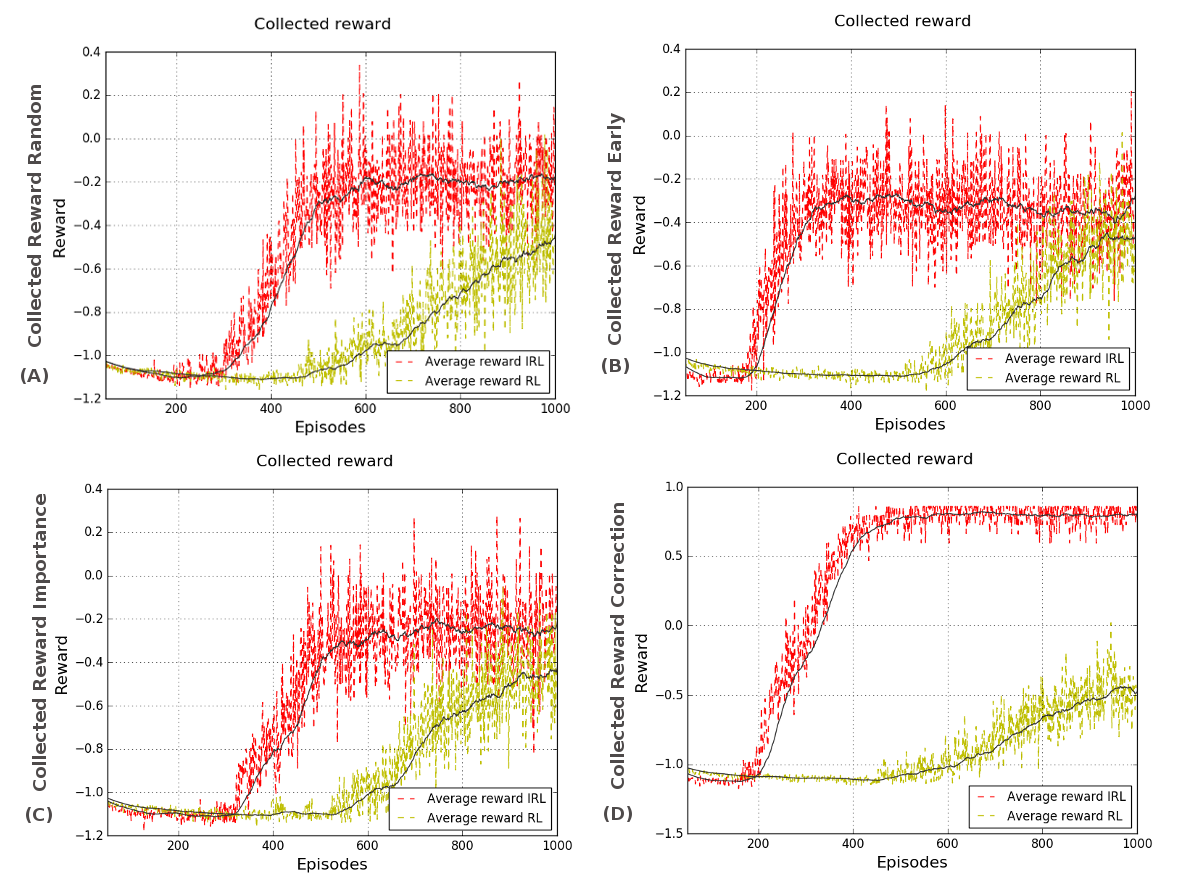
\includegraphics[scale=0.5]{collected_reward_results.png}     
      \caption{\scriptsize Average accumulated reward achieved by 30 simulated student-teacher pairs over a duration of 1000 episodes with a static feedback probability of 0.3 (A), early advising (B), importance advising (C), and mistake correcting (D). The green dotted line represents the autonomous learning process of the teacher agents, the red dotted line the learning process of the student using IRL.}
      \label{collectedrewardresults}
\end{figure}

For the early advising, we set the advice budget per episode to 3, so that the teacher would give advice for exactly the first 3 steps of each episode and never afterwards. This adds up to exactly 3000 instances of advice-giving throughout all episodes, slightly less than the amount random advising ended up giving. The average rewards obtained this way are shown in Figure \ref{collectedrewardresults}. We can see that the student agent actually learns much quicker initially, already acquiring an average reward of roughly -0.3 after 400 episodes. On the flip side however, its behaviour does not improve significantly anymore even after 600 additional episodes, whereas the random advice approach eventually reaches an average reward of just over -0.2. This seems to be in line with the philosophy of the early advising strategy: The student is quickly brought on the right track at the beginning of each episode, but when exploring optimized solutions during later stages of the episodes is left completely on its own and produces worse results. Nevertheless, this could be useful for developing some kind of hybrid strategy, where early advising is gradually transformed into a more far-sighted approach as the number of episodes grows. Also, in the context of a possible human teacher working with a learning robot, this strategy is very easy and intuitive to apply.
\\
The next strategy we wanted to try was importance advising, as it seemed to have a great effect on the problems introduced by Taylor et al. (\cite{Taylor2014reinforcement}). We chose as importance function the mean absolute deviation of Q-values for the particular state as observed by the teacher. This way, we hoped to focus advice on states that making mistakes in would be especially bad and to let the student make less impactful decisions by itself to preserve the budget. Finding the right threshold for the importance function proved to be non-trivial: If chosen too low, the strategy starts to closely resemble early advising; if chosen too high, the total amount of advice gets too low to allow for a fair comparison with the other approaches. We ended up with a threshold of 0.02 for the absolute deviation of Q-values, which resulted in approximately 3000 instances of the teacher giving advice throughout all episodes. The resulting average rewards can be seen in Figure \ref{collectedrewardresults}. Disappointingly, this approach does actually not seem to perform any better than the random method with a comparable amount of advice. The initial learning process is not accelerated significantly, and the average reward after 1000 episodes of training is slightly lower. A reason for this could be the fact that there is actually only the rather small number of 46 regular states that are not either the goal state or result in immediate failure. This, combined with the fact that the typical episode does not last very long, could result in the teacher giving advice in the same states over and over, even if the student has already developed the correct policy for those cases.
\\
The natural answer for this problem, as introduced by Taylor et al. in \cite{Taylor2014reinforcement}, would be to only give advice to the student if that advice actually leads it to perform a different action than what it otherwise would have. This mistake correcting approach is a direct extension of importance advising: Advice still only gets considered if the current state is deemed important by the teacher, but now the student's decision also has to actually differ from the teacher's in order to prompt a reaction. Running the scenario as a simulation, we are in the fortunate position of being able to predict the student's decision without actually having to let them perform it first, which makes the implementation of this approach a lot less complicated. Figure \ref{collectedrewardresults} shows average obtained rewards of agents trained using this interactive approach. Not only is the initial learning process of the agents significantly faster than with random advising, the final learning result shows a great difference to any of the other approaches as well. The average reward achieved after 1000 episodes ends up at about 0.81, where random advising would be at around -0.2 accumulated reward per episode. In comparison, the theoretical maximum reward per episode that can be achieved is 0.86, in an episode of 15 actions. The majority of agents thus actually learns the optimal policy to fulfill the task in 15 actions this way, even if taught by an agent that is not even close to achieving the same itself. We can see this effect in Figure \ref{stepsfailurescorrection}, where the average amount of actions per episode is being shown. The shorter average episodes from the earlier stages of the learning process result from the fact that these runs often end up in failure states. The positive influence on the quality of the learned policy using mistake correcting is further confirmed when comparing the average amount of total advice which for mistake correcting is only around 1800, so roughly 2 instances per episode. \\

Of course, the additional power of having a mistake correcting mechanism comes at a price: To reliably correct mistakes, we need to either wait for them to actually happen, or we need to know ahead of time what decision the student is going to take. Both approaches pose problems when we look at a real world application instead of a simulation: We often cannot simply tell a robot to "undo" its last action and do something else after it has already been performed, like when it tries to clean the table with a cup and crushes it in the process. Likewise, if we want to know the next action beforehand, the robot needs to constantly communicate about its plans and wait for possible feedback before actually executing anything. This is theoretically possible, especially if the amount of possible actions is rather low and abstract like in our simulation. For more complex scenarios with more or more parameterized actions, this could slow the learning process down considerably just by executing way fewer actions in the same amount of time. A "pure" mistake correction strategy would probably not be feasible in those cases, but the concept is definitely always worth thinking about when looking at interactive reinforcement learning tasks.

\begin{figure}[H]
      \centering
      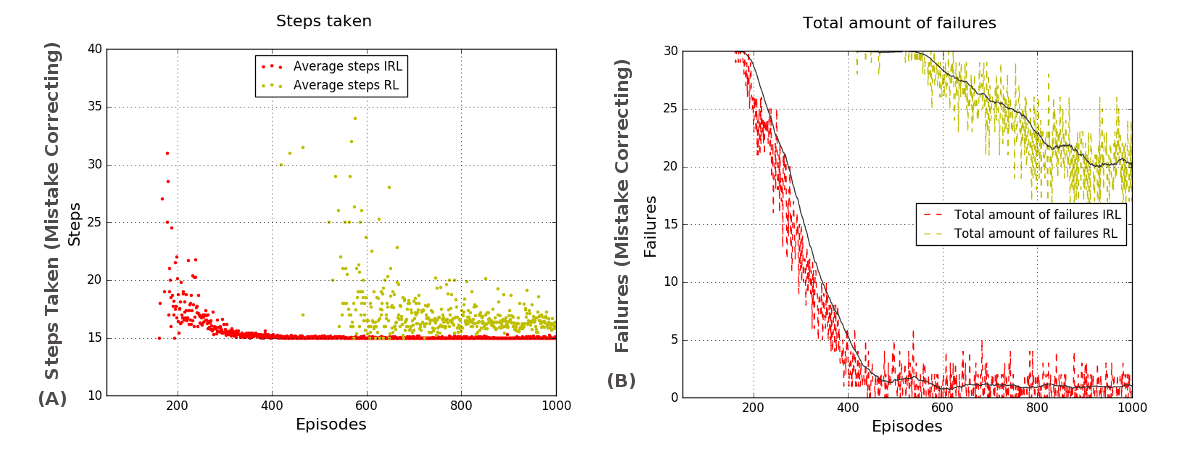
\includegraphics[scale=0.5]{steps_failures_correction.png}     
      \caption{\scriptsize Figure 3 Description - Steps Failures Correction.}
      \label{stepsfailurescorrection}
\end{figure}

\section{Conclusion}

After giving an introduction to reinforcement learning and its basics we have expanded the general approach to include the idea of a learning process that is autonomous, but assisted by a teacher giving continuous advice throughout the learning process. We introduced a selection of approaches that aim to find efficient implementations for this concept which can be used in a real-world scenario and discussed their advantages and disadvantages for certain problem domains. Finally, we took a closer look at the idea of advice budgets and how to efficiently act as a teacher when the amount of allowed feedback is limited. We implemented a selection of different strategies in a scenario based on \cite{cruz2014improving} and evaluated their performance. We can conclude that choosing an appropriate advice strategy can be crucial in allowing the RL process to achieve much better results in a shorter period of time, however, strategy-specific implications can also introduce strong restrictions on the system as a whole. Thus, the choice of strategy should be carefully considered in regards to application-specific properties.


\label{sec:concl}

%%%%%%%%%%%%%%%%%%%%%%%%%%%%%%%%%%%%%%
% hier werden - zum Ende des Textes - die bibliographischen Referenzen
% eingebunden
%
% Insbesondere stehen die eigentlichen Informationen in der Datei
% ``bib.bib''
%
\newpage
\bibliographystyle{plain}
\addcontentsline{toc}{section}{Bibliography}% Add to the TOC
\bibliography{bib}

\end{document}


